\documentclass{article}
\usepackage{fontspec}
\usepackage{type1cm}
\usepackage{geometry}
\usepackage[bold-style=ISO]{unicode-math}
\usepackage[heading=true]{ctex}%添加heading=true,使用中文版式
\usepackage{graphicx}
\geometry{a4paper,left=1cm,right=1cm,top=1cm,bottom=1cm}
\begin{document}
\begin{flushleft}
	\fontsize{24pt}{30pt}\selectfont
	~\\ \textbf{定积分} \\~\\
	定积分是一个特殊的极限\\
	$\int_{a}^{b}f(x)dx=\lim\limits_{\lambda\to 0}\sum_{i=1}^{n}f(\xi_i)\Delta x_i$\\
	其中$\lambda = max\{\Delta x_1, \Delta x_2...\Delta x_n\}$\\
	\ \ $\Delta x_i=x_i-x_{i-1}$\\
	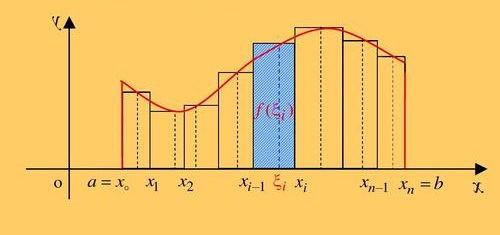
\includegraphics[scale=1.0]{2.jpg}\\
	~\\
	定积分的几何意义:曲边梯形的面积的代数和\\
	~\\
	若$f(x)$在$[a,b]$上连续,则$f(x)$在$[a,b]$上可积\\
	若$f(x)$在$[a,b]$上有界,且只有有限个间断点,则$f(x)$在$[a,b]$上可积\\
	~\\ \textbf{定积分的性质} \\~\\
	1.等式性质\\
	\ \ $\int_{a}^{a}f(x)dx=0$\\
	\ \ $\int_{a}^{b}f(x)dx=-\int_{b}^{a}f(x)dx$\\
	\ \ $\int_{a}^{b}[\alpha f(x)\pm \beta g(x)]dx=\alpha\int_{a}^{b}f(x)dx\pm \beta\int_{a}^{b}g(x)dx$\\
	\ \ $\int_{a}^{b}f(x)dx=\int_{a}^{c}f(x)dx+\int_{c}^{b}f(x)dx$\\
	2.不等式性质(前提$b>a$)\\
	\ \ 设$f(x)\le g(x)$,则$\int_{a}^{b}f(x)dx\le \int_{a}^{b}g(x)dx$\\
	\ \ 设$f(x)\ge 0$,则$\int_{a}^{b}f(x)dx \ge 0$\\
	\ \ $|\int_{a}^{b}f(x)dx| \le \int_{a}^{b}|f(x)|dx$\\
	\ \ 设$m<f(x)<M$,则$m(b-a)<\int_{a}^{b}f(x)dx<M(b-a)$\\
	3.积分中值定理\\
	设$f(x)$在$[a,b]$上连续,则$\exists \xi \in [a,b]$或$\exists \xi \in (a,b)$,使得$\int_{a}^{b}f(x)dx=f(\xi)(b-a)$\\
	~\\
	使用定积分定义求极限:$\int_{0}^{1}f(x)dx=\lim\limits_{x\to \infty}\frac{1}{n}\sum_{i=1}^{n}f(\frac{i}{n})$\\
	
\end{flushleft}
\end{document}